\documentclass[a4paper,12pt]{article}
%%%%%~~~~~~~~~~~~~~~~~~~~~usepackage~~~~~~~~~~~~~~~~~
\usepackage{rotating}
\usepackage[top=1in, bottom=1in, left=1in, right=1in]{geometry}
\usepackage{graphicx}
\usepackage[numbers,square,sort&compress]{natbib}
\usepackage{setspace}
\usepackage[cdot,mediumqspace,]{SIunits}
\usepackage{caption}
\usepackage{subcaption}
\usepackage{mathtools}
\usepackage{authblk} % to get affil
\usepackage{float} % to get figures where wanted
\usepackage{indentfirst} % to indent the first para of every chapter


%####################### new command

\newcommand{\myemail}{ayushi.singh@mail.utoronto.ca}
\newcommand{\anita}{anita.bahmanyar@mail.utoronto.ca}
\newcommand{\carly}{c.berard@mail.utoronot.ca}

%####################### Title and etc

\begin{document}
\onehalfspacing
\title{Photon Counting and the Statistics of Light}
\author{Ayushi Singh, Anita Bahmanyar, Carly Berard}
\affil{\small {\myemail}}%, {\anita}, {\carly}}
\affil{\small Astronomy and Physics, University of Toronto, ON}
\date{30 September, 2013}
\maketitle
%\altaffiltext{1}{{\myemail}}
%\altaffilmark{1}
%####################### Abstract

\begin{abstract}
\label{abstract}
This experiment examined the distribution of photon collected using PMT for different number of samples and time intervals. Python programming language was used to calculate mean and standard deviation, and to plot the graphs and histograms. Various time vs. count plots show that increasing number of samples give us more precise counts per sample, where as, increasing the time intervals widens the range of count per sample. The shape of histograms (frequency vs. count graphs) and mean vs. variance graphs strongly support Poisson distribution, even at higher time intervals. It is also induced that with large number of samples ${N}$, precision of a measurement of mean increased  by the factor of $\sqrt{N}$. 
\end{abstract}

%####################### Introduction
\section{Introduction}
\label{sec:introduction}
The purpose of this report is to discuss the physical limitation of detecting light. The two main parameters: Number of samples and time interval was explored. Photons collected through PMT with these parameter produce a histogram that fits the poisson distribution. In this report, this idea was tested and compared to other distributions. The report also investigate the fundamental statistics and plots created using Python.

%####################### Equipment
\section{Equipment and Method}
\label{sec:equipment}
Photomultipler Tube (PMT) was used to collected the data. It is a black box that receive photon and uses photoelectric effect to multiply the number of photons. PMT outputs a pulse \citep{PMT}. Using the python script (PMT Python Module \citep{Module}), provided in advance, number of counts per sample was recored. This depends on the two parameters: number of samples and time interval, which is specified before running the PMT.

%####################### Data
\section{Data Summary}
\label{sec:data}

The data collected from PMT using PMT Python Module was represented in python array of counts per sample and saved in a file. These files were then later used to manipulate the data. Multiple data was collected with different time interval and number of samples using the method explained in Section \ref{sec:equipment}. For each combination number of samples and time interval, 6 or 10 data set was collected. 


\begin{table}[H]
\centering % used for centering table
\caption{Summary of all the data collected for the experiment}
\tabcolsep 2.pt %\small
\footnotesize

\begin{tabular}{ccccc}% centred columns (8 columns)
\hline
\hline

Data Number  & Time Interval & Number of Samples & Number of data set & Comments \\
& (s) & & &\\

 
\hline
\hline
1   &   0.001   &   100     &   6   & \\
2   &   0.01    &   400     &   6   & \\
3   &   0.01    &   400     &   6   & comparing mean and variance \\
4   &   0.0125  &   400     &   6   & comparing mean and variance \\
5   &   0.025   &   400     &   6   & comparing mean and variance \\
6   &   0.0375  &   400     &   6   & comparing mean and variance \\
7   &   0.05    &   400     &   6   & comparing mean and variance \\
8   &   0.08    &   400     &   6   & comparing mean and variance \\
9   &   0.1     &   400     &   6   & comparing mean and variance \\
10  &   0.001   &   1000    &   6   & for theoretical distribution\\
11  &   0.1     &   1000    &   6   & for theoretical distribution\\
12  &   0.001   &   2       &   10  & exploring MOM and SDOM\\
13  &   0.001   &   4       &   10  & exploring MOM and SDOM\\
14  &   0.001   &   8       &   10  & exploring MOM and SDOM\\
15  &   0.001   &   16      &   10  & exploring MOM and SDOM\\
16  &   0.001   &   32      &   10  & exploring MOM and SDOM\\
17  &   0.001   &   64      &   10  & exploring MOM and SDOM\\
18  &   0.001   &   128     &   10  & exploring MOM and SDOM\\
19  &   0.001   &   256     &   10  & exploring MOM and SDOM\\
20  &   0.001   &   512     &   10  & exploring MOM and SDOM\\
21  &   0.001   &   1024    &   10  & exploring MOM and SDOM\\
22  &   0.001   &   2048    &   10  & exploring MOM and SDOM\\
23  &   0.001   &   100     &   6   & dark count\\
24  &   0.001   &   1000    &   6   & dark count\\
25  &   0.01    &   400     &   6   & dark count\\
\hline
\hline

\end{tabular}
\label{table:dataset} % is used to refer this table in the text
\end{table}

%####################### Data Reduction
\section{Data Reduction}
\label{sec:reduction}

Most of the data collected went though two main methods of calculating mean and standard deviation. These are used in later sections for analyzing and understanding the behaviour of data. 

\begin{equation}
\label{eq:mean}
\mu = \frac{\sum x_i}{N},
\end{equation}
where $\mu$ is the mean and $N$ is number of samples. This is the average value of the data.

\begin{equation}
\label{eq:SD}
\sigma = \sqrt{\frac{\sum x_i - \mu}{N-1}},
\end{equation}
where $\sigma$ is the standard deviation. This value represents the uncertainty in the measurement for that data set. 

%####################### Discussion 
\section{Discussion}
\label{sec:discussion}

%####################### light
\subsection{Variation in light count} 
\label{sec:light}

Each data file had list of counts per sample, as mentioned in Section \ref{sec:data}. The data from the Table \ref{table:dataset} is used to graph time vs count plots and histograms as followed:
%~~~~~~~~~~~~~~~~~~~~~~~~~~~~~~~~~~~~~~~~~~~~~~~~~~~
\begin{figure}[H]
\centering
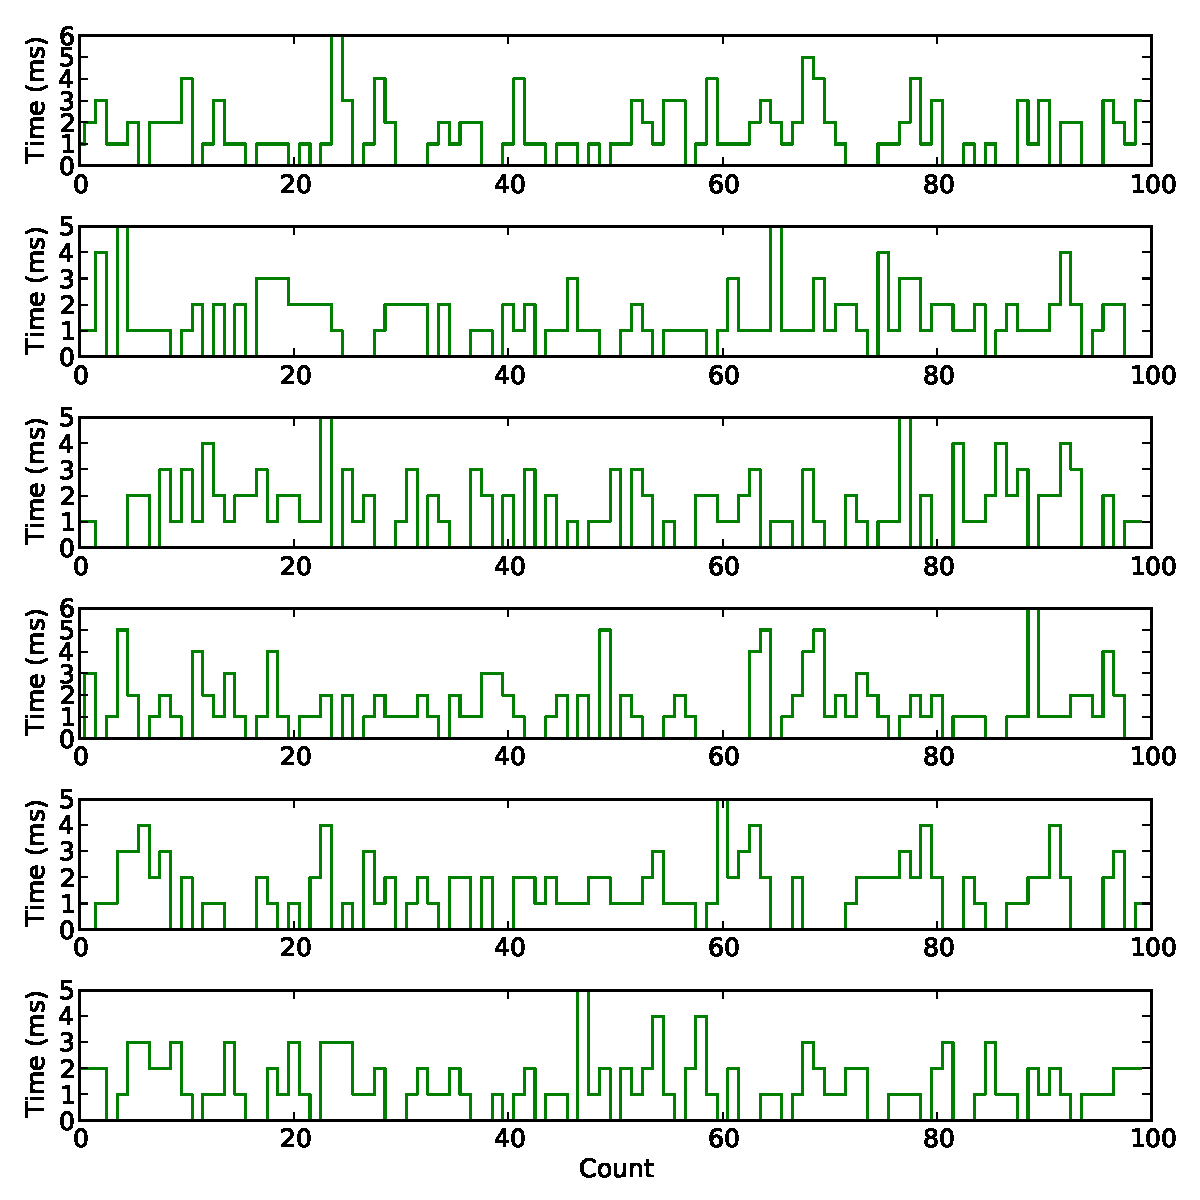
\includegraphics[angle=0,height=12cm,width=15.5cm]{graphs/task1.pdf}
\caption{Time vs. count per sample graph for data number 1 from Table \ref{table:dataset}. There are six sets of data, where time interval of each sample is 0.001s for 100 samples.}
\label{fig:task1_plots}
\end{figure}

\begin{figure}[H]
\centering
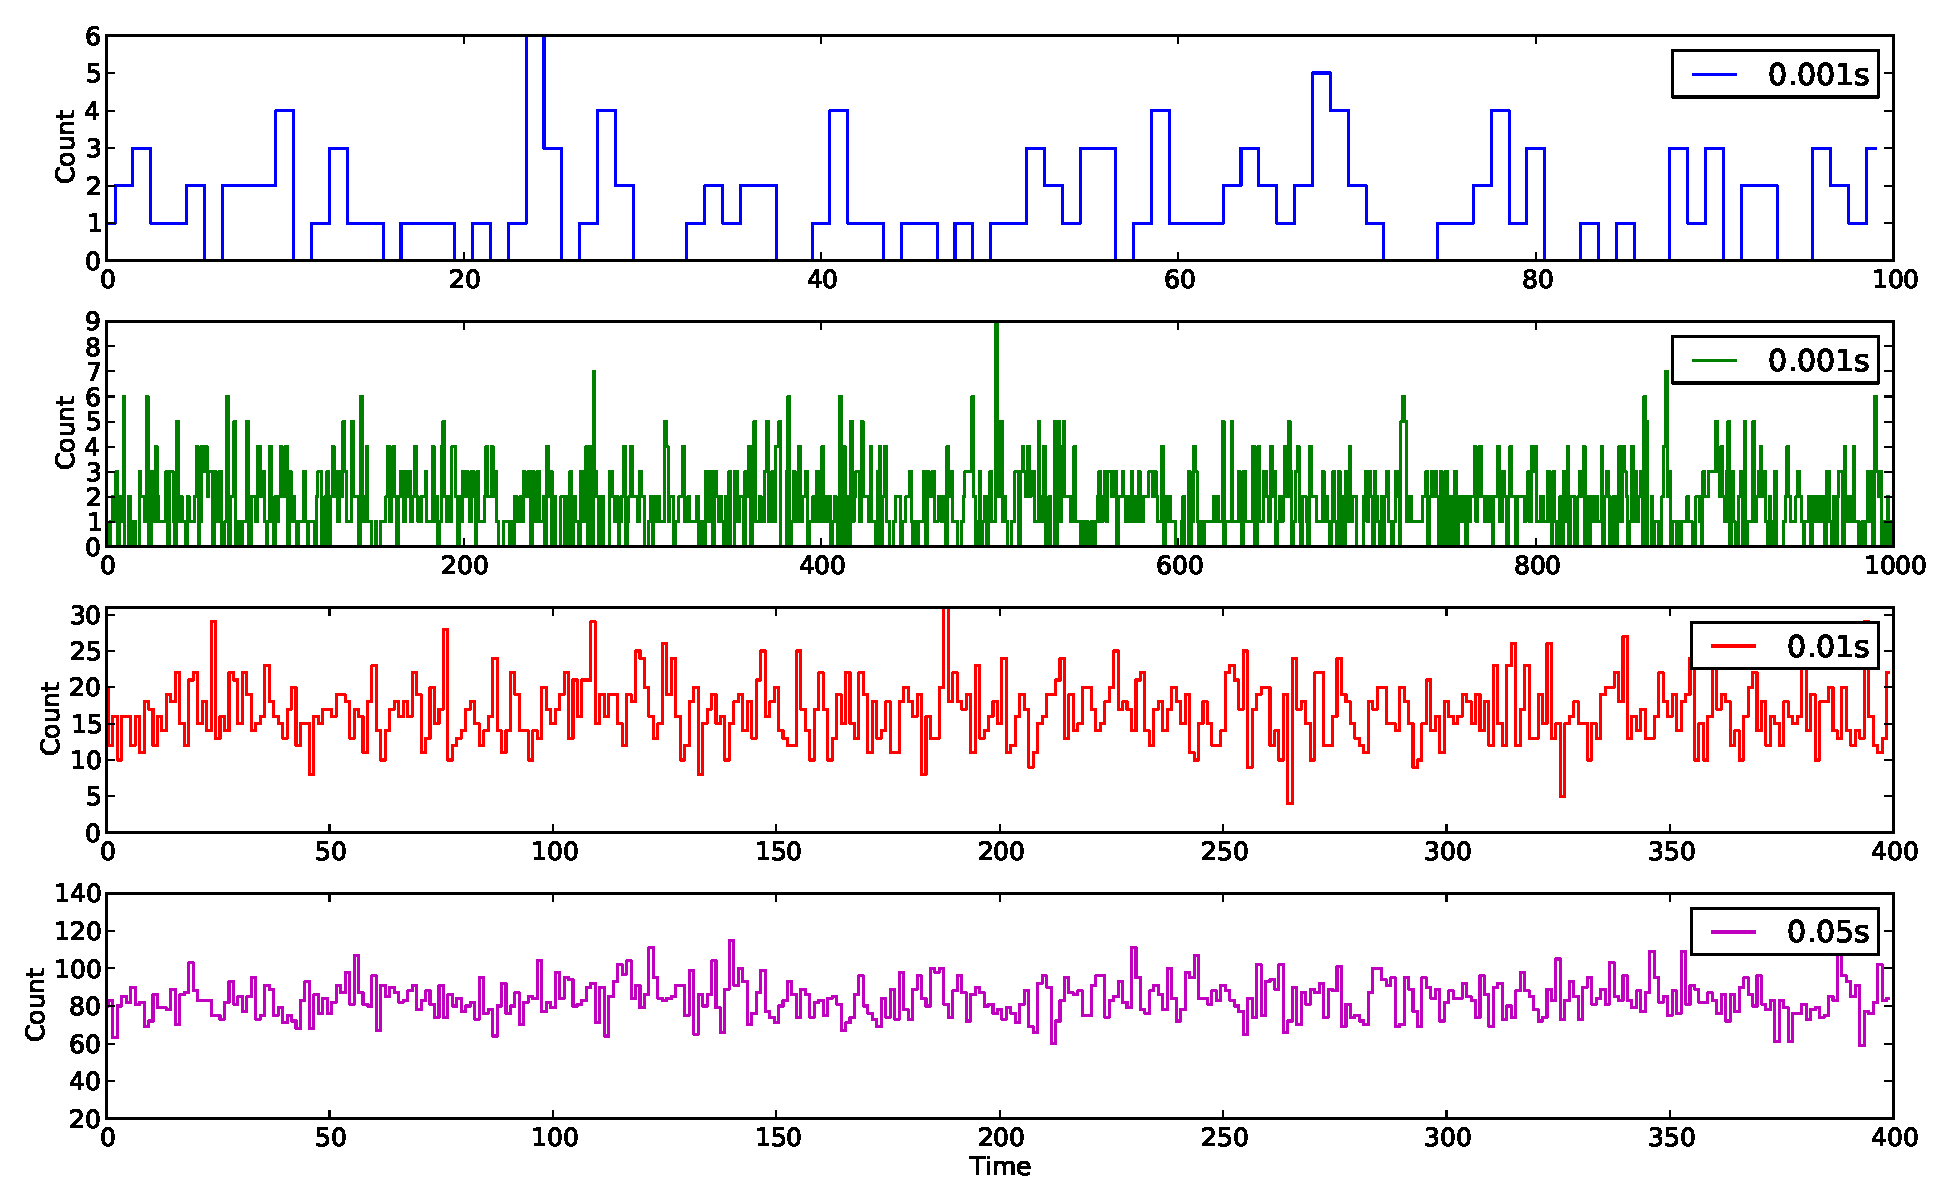
\includegraphics[angle=0,height=11cm,width=15.5cm]{graphs/diff_plots.pdf}
\caption{Time vs. count per sample graph for data number 1, 3, 7 and 10 from Table \ref{table:dataset}. Only one of each set is used. Blue and green graphs show affect of change in sample numbers, where as, red and magenta graphs show variation by changing time interval.}
\label{fig:diff_plot}
\end{figure}

\begin{figure}[H]
\centering
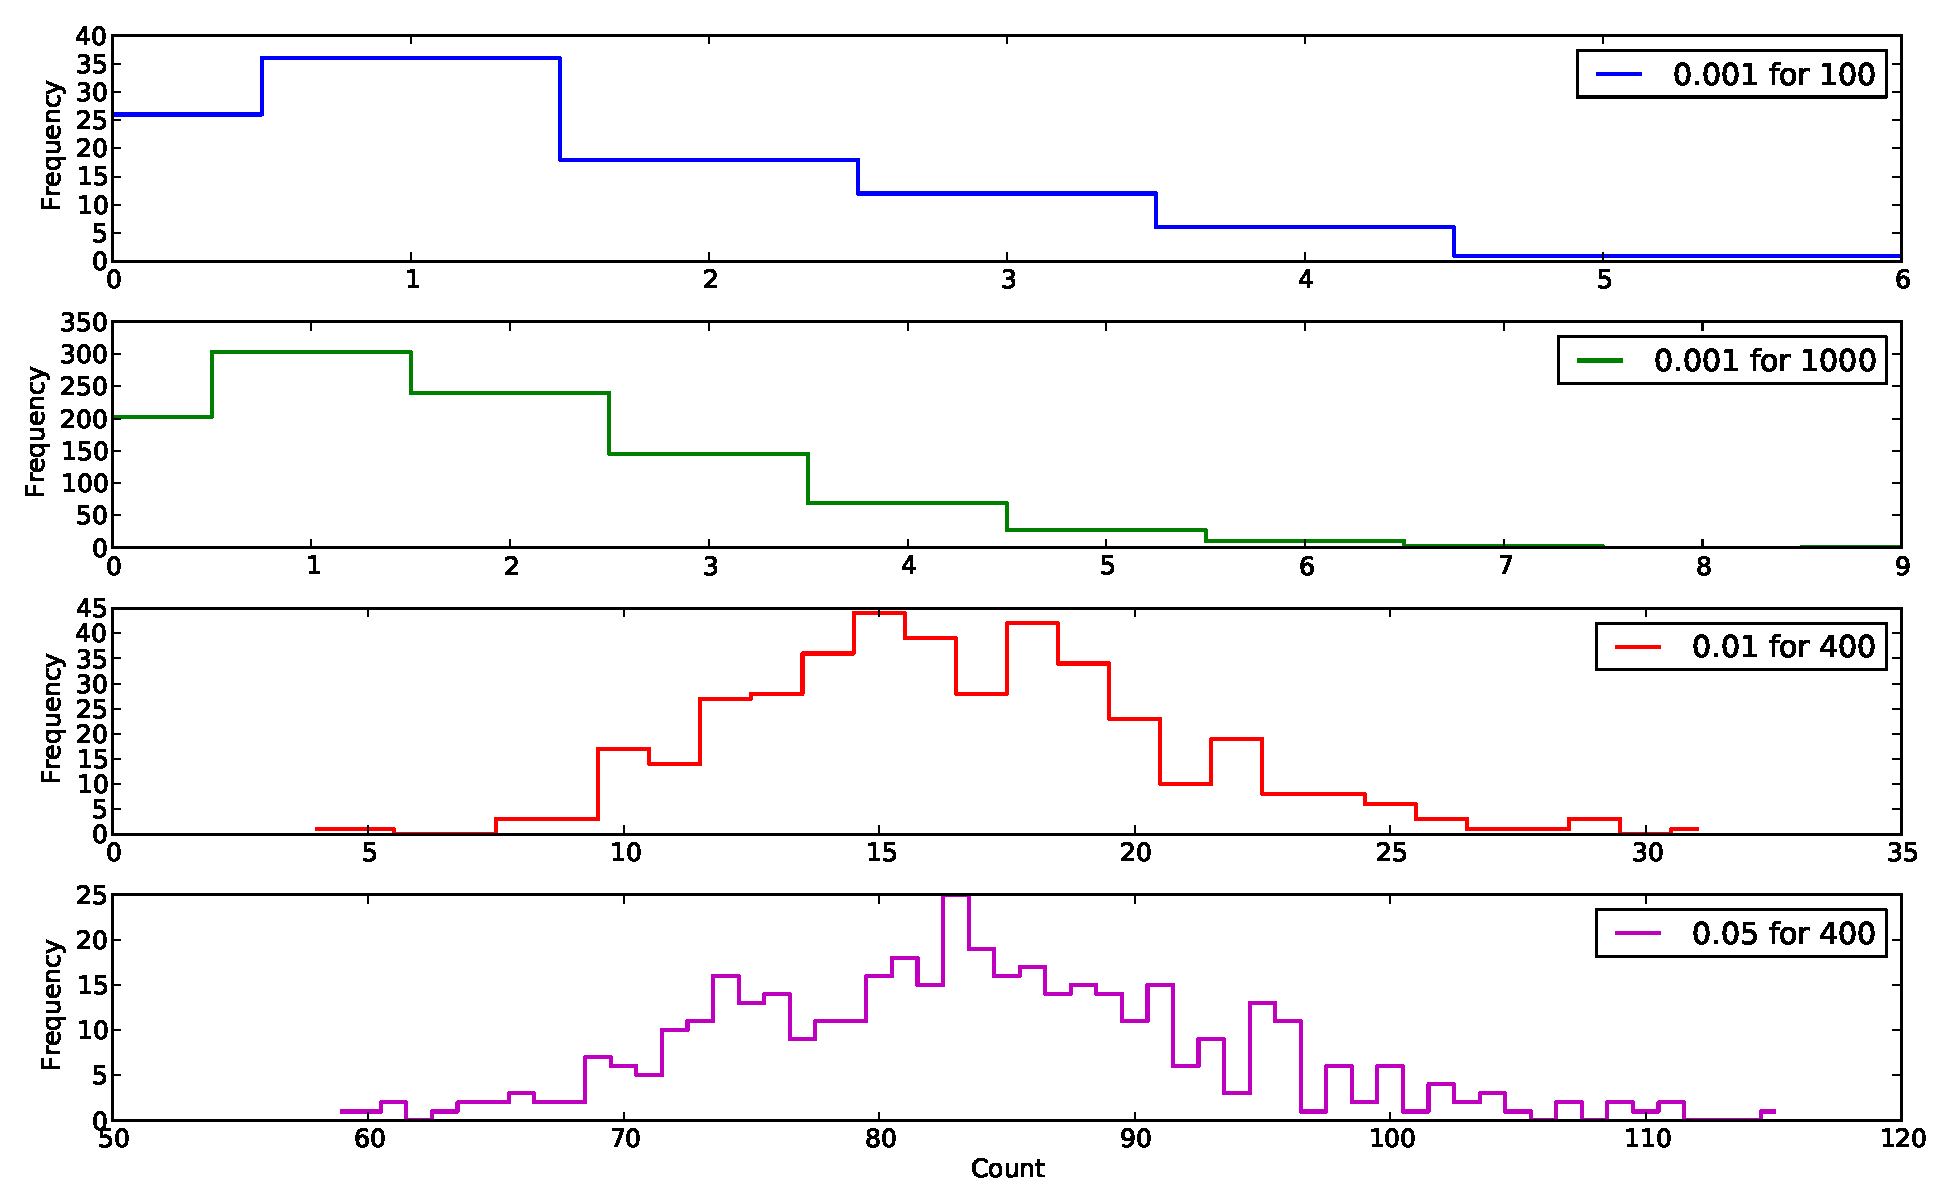
\includegraphics[angle=0,height=10cm,width=15.5cm]{graphs/diff_hist.pdf}
\caption{Histogram of data plotted in Figure \ref{fig:diff_plot}}
\label{fig:diff_hist}
\end{figure}

%~~~~~~~~~~~~~~~~~~~~~~~~~~~~~~~~~~~~~~~~~~~~~~~~~~~
The Figure \ref{fig:task1_plots} shows that even with a same time interval and number of samples, data obtained in these 6 set is quite dissimilar, that is, no two plots look alike. This exhibits that PMT gives out photons, randomly and within a range of values. In this case, the range of count is from 0-6. However, there is a peak value that occurs more often.   

\begin{table}[H]
\centering % used for centering table
\caption{Calculated values for light count}
\tabcolsep 2.pt %\small
\footnotesize

\begin{tabular}{cccc}% centred columns (8 columns)
\hline
\hline

Plot colour  & Mean & Standard Deviation & Count rate \\
& & &(Hz)\\ 
\hline
\hline
Blue&  1.43 &   1.30 & 1430\\
Green&  1.71&  1.40&  1710\\
 Red &16.51   &   4.14 & 1651\\
 Magenta & 83.78  &  9.63 & 1676\\
\hline
\hline

\end{tabular}
\label{table:light} % is used to refer this table in the text
\end{table}

Figure \ref{fig:diff_plot} and \ref{fig:diff_hist} shows the change that occur by chaining two parameters. Blue and green plot displays that by increasing the number of samples from 100 to 1000, the range of count is increased to 0-9, even though the time interval is unchanged. There are samples with count as high as 9 in green plot, where as in blue plot the maximum is only 6. This increases the precision of the result that can be seen in Table \ref{table:light}. Red and magenta plots, on the other hand, deal with fixed number of samples and change in time interval from 0.01s to 0.05s. In Figure \ref{fig:diff_plot}, it is explicit that more photons are detected per sample by increasing the time interval, as can be seen from the mean value in Table \ref{table:light}. However, this widens the range of count per sample, even though, numbers of sample for both is 400. As exhibited in Figure \ref{fig:diff_hist}, 15 counts occurred 45 time at 0.01s. Where as, at 0.05s, only 82 counts occurred only 25 time. In the Table \ref{table:light}, the count rate value increases with the increase in both the parameters.

%####################### Dark
\subsection{Effect of Dark Count}
\label{sec:dark}
Dark counts are counts taken using PMT with lights off. This generates a similar plots but as light counts (PMT with light on), but they are different in the values they provide us. This shows that PMT is not perfect black box and detects photons even when the lights are off. This is considered noise. %~~~~~~~~~~~~~~~~~~~~~~~~~~~~~~~~~~~~~~~~~~~~~~~~~~~
\begin{table}[H]
\centering % used for centering table
\caption{Calculated values for dark count}
\tabcolsep 2.pt %\small
\footnotesize

\begin{tabular}{ccccc}% centred columns (8 columns)
\hline
\hline

Plot colour  & Mean & Standard Deviation & Count rate \\
& & &(Hz)\\ 
\hline
\hline
Blue&  0.56 &   0.76 & 560\\
Green&  0.49&  0.69&  490\\
 Red & 5.21   &   2.31& 521\\
\hline
\hline


\end{tabular}
\label{table:dark} % is used to refer this table in the text
\end{table}

\begin{figure}[H]
\centering
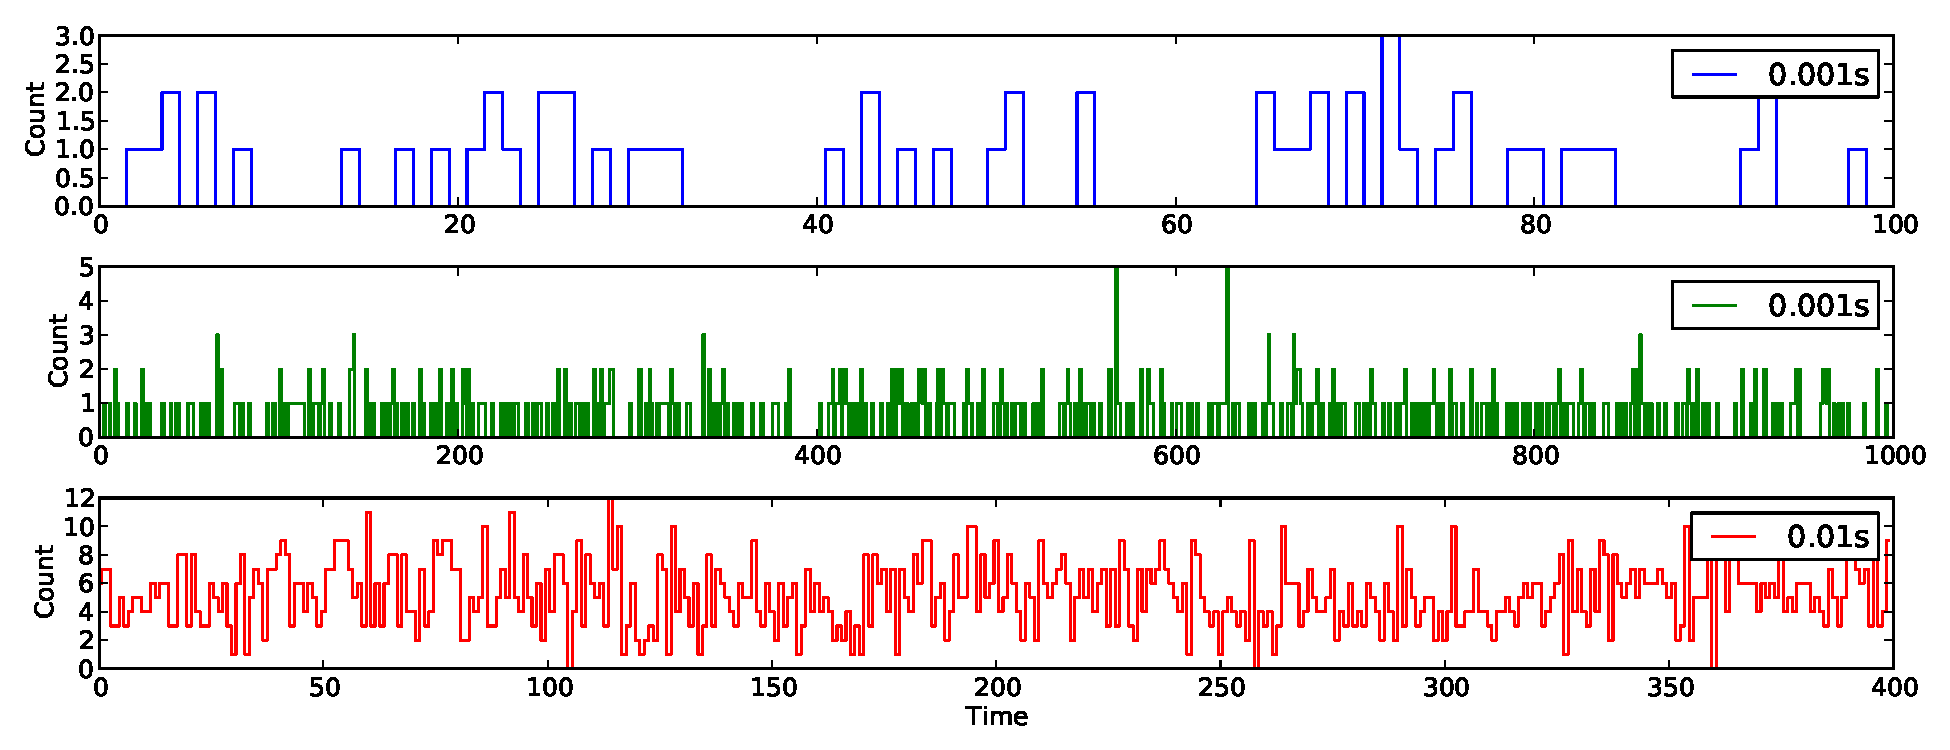
\includegraphics[angle=0,height=8cm,width=15.5cm]{graphs/dark_plots.pdf}
\caption{Time vs. count per sample graph for dark count  for three different set of data for Figure \ref{fig:diff_plot} and Figure \ref{fig:diff_hist}. This is from data number 23, 24 and 25 from Table \ref{table:dataset}}
\label{fig:dark_plot}
\end{figure}

\begin{figure}[H]
\centering
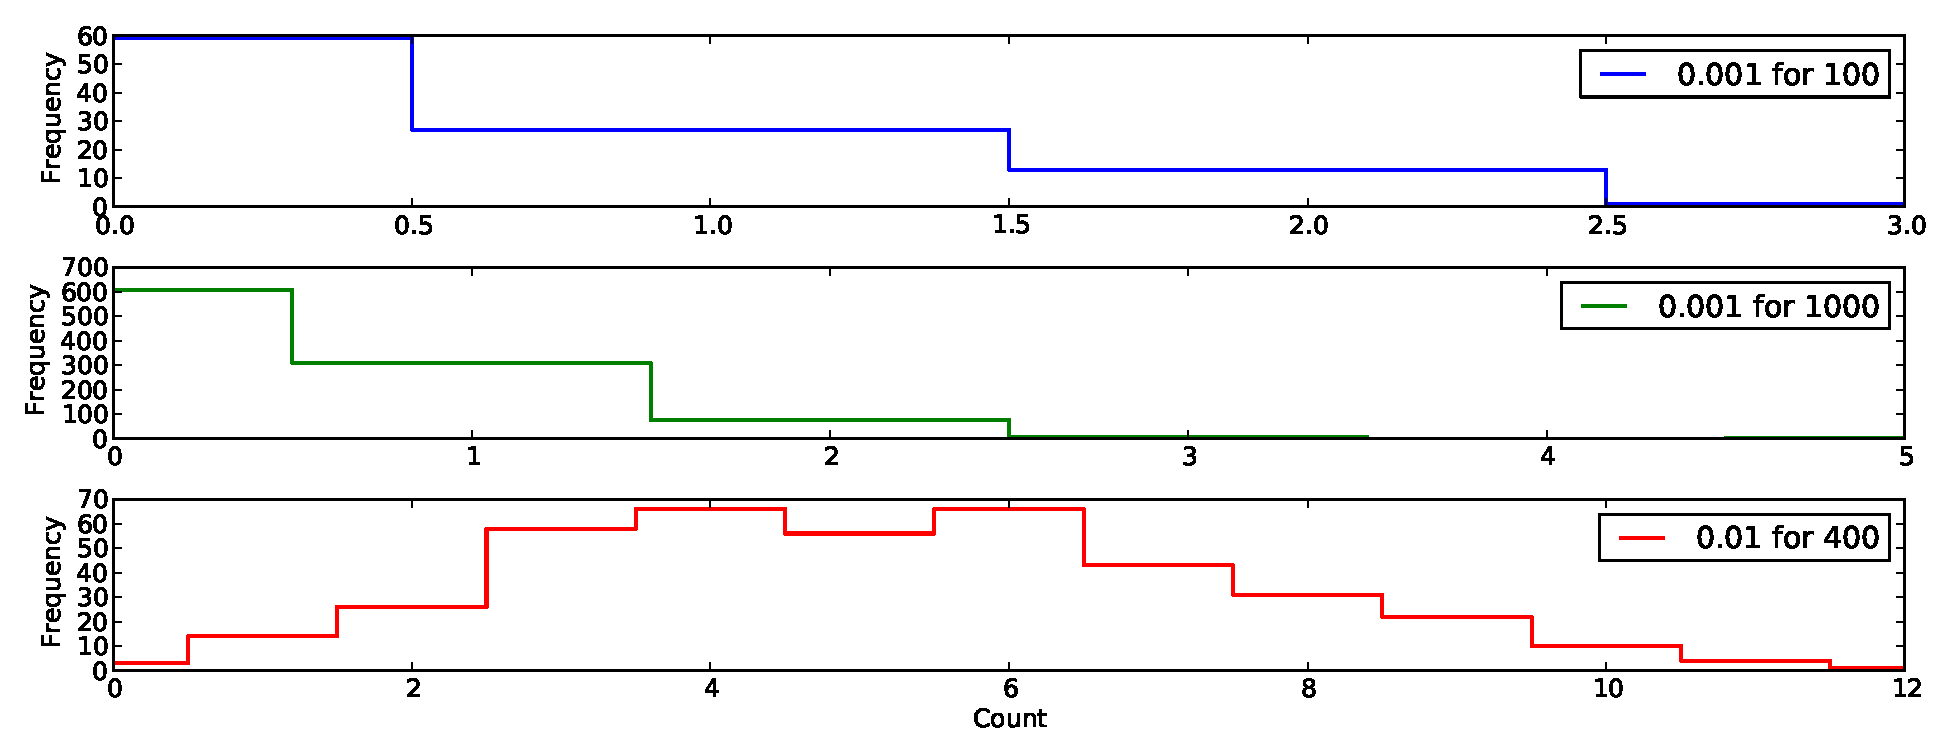
\includegraphics[angle=0,height=8cm,width=15.5cm]{graphs/dark_hist.pdf}
\caption{Histogram of data plotted in Figure \ref{fig:dark_plot}.}
\label{fig:dark_hist}
\end{figure}


%~~~~~~~~~~~~~~~~~~~~~~~~~~~~~~~~~~~~~~~~~~~~~~~~~~~
From Figure \ref{fig:dark_plot} and \ref{fig:dark_hist}, it is clear that there is some noise in the PMT. Blue and green plots have more counts at zero where time is 0.001s. However, in red plot, there is a peak at 4 and 6 count showing that by increasing the time to 0.01s, more noise was introduced. There are few factors that could have contributed to this noise. PMT is not perfect black box and some of the photons from outside were detected. Another contributor to the noise could possibly be the internal heat of the PMT. Upon heating up, the PMT could have released photons that were detected. It explains the larger mean and standard deviation for red and green compared to blue in Table \ref{table:dark}. PMT is working for longer period of time. 

%####################### count rate 
\subsection{Count rates of different sample}
\label{sec:countrate}

Data number 1and 2 from Table \ref{table:dataset} is 6 sets of data for 100 and 400 number of samples, respectively . It was used to calculate mean and standard deviation for every data set using Equation \ref{eq:mean} and \ref{eq:SD}. Count rate was calculated by $\frac{mean}{time\;interval}$. Then the mean and standard deviation of the 6 count rates for each set was calculated using same equation. The mean and standard deviation of count rate is:
\begin{itemize}
\item For 100 number of samples: 1366.67 and 43.20
\item For 400 number of samples: 1664.67 and 18.09
\end {itemize}
From the result it clear that by increasing the number of samples, higher count rate can be obtained with smaller standard deviation. 


%####################### mean and variance
\subsection{Relationship between mean and variance}
\label{sec:meanandvariance}
Data number 3-9 from Table \ref{table:dataset} was used to calculate and analyze the relationship between the mean and variance. Mean is calculated using Equation \ref{eq:mean}. And variance is standard deviation squared \citep{Stat}; therefore, it is $\sigma^{2}$, where sigma is from Equation \ref{eq:SD}. 
%~~~~~~~~~~~~~~~~~~~~~~~~~~~~~~~~~~~~~~~~~~~~~~~~~~~
\begin{figure}[H]
\centering
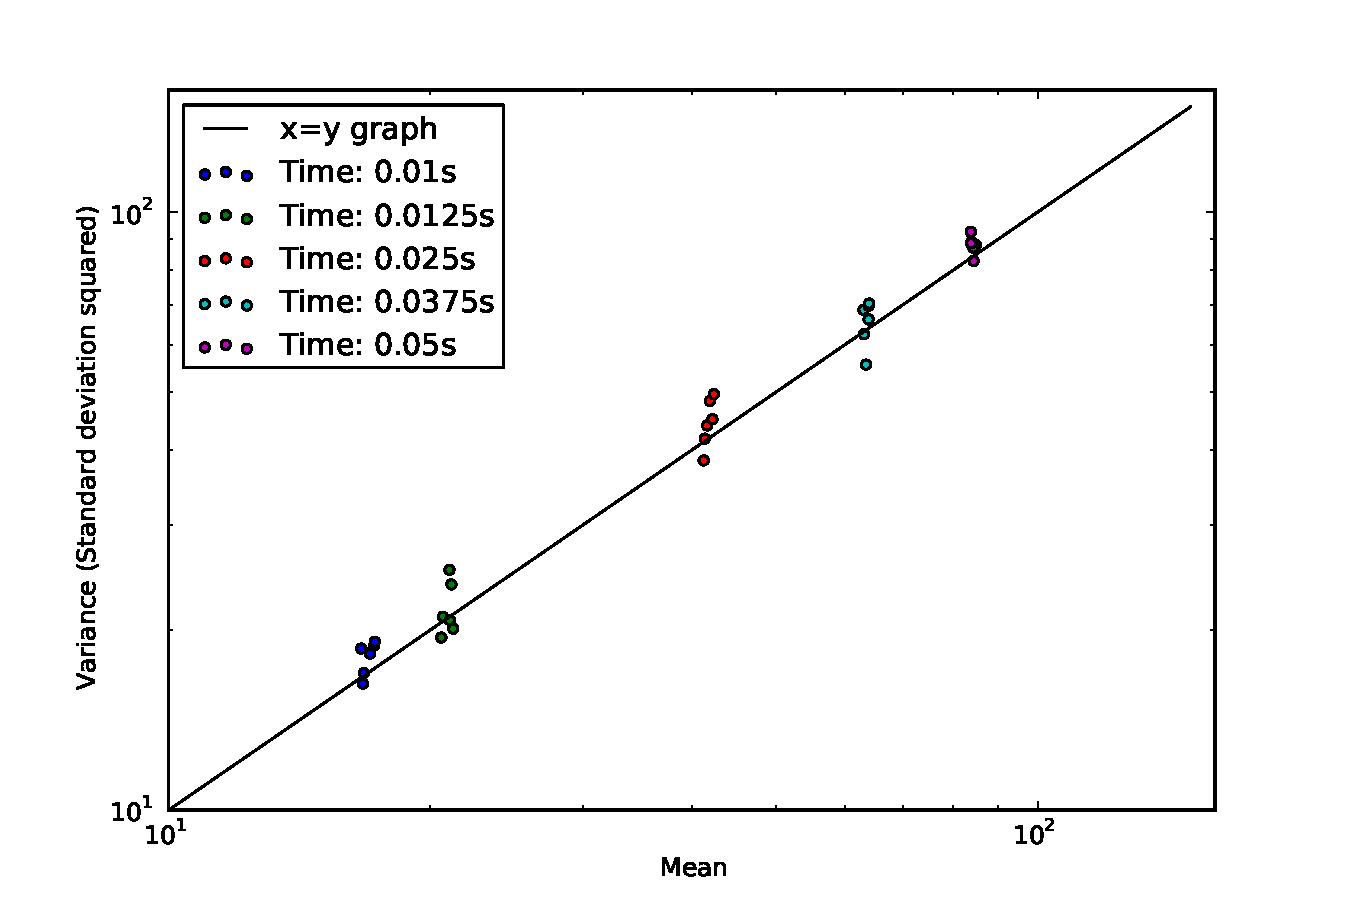
\includegraphics[angle=0,height=9.5cm,width=15.5cm]{graphs/Task7_log-log.pdf}
\label{fig:task7log}
\caption{Mean vs. Variance (standard deviation squared) log-log graph. The sample size for all the data is 400. There are six sets of data for each of seven different time interval.}
\end{figure}
%~~~~~~~~~~~~~~~~~~~~~~~~~~~~~~~~~~~~~~~~~~~~~~~~~~~
Data here have 400 number of sample each but various in time interval. The log-log graph (Figure 6) of mean vs. variance clearly show a linear relationship. The line $y=x$ runs through the middle of the data points, even for the large number. That is, as the time interval increases the mean and the variance increases with linear proportionality. This can be interpreted as property of poisson distribution \citep{Stat}, where mean is equal to variance. 

%####################### theoretical prediction
\subsection{Comparing results with theoretical distribution}
\label{sec:theoretical}
From the Table \ref{table:dataset}, data number 10 and 11 were used to plot histogram, poisson distribution and gaussian distribution.

\begin{equation}
\label{eq:poisson}
P(x;\mu) = \frac{\mu^x}{x!}\exp(-\mu),
\end{equation}
where $\mu$ is the mean and $x = 1, 2, 3 ...$. This equation describes the poisson distribution. It has discrete value \citep{Stat}. 

\begin{equation}
\label{eq:gaussian}
P(x;\mu;\sigma) = \frac{1}{\sigma \sqrt{2\pi}}\exp \left[-\frac{1}{2} \left(\frac{x - \mu}{\sigma} \right)^2 \right],
\end{equation}
where $\mu$ is the mean and $\sigma$ is the standard deviation. This is equation for gaussian distribution and it is continuos distribution \citep{Stat}.

%~~~~~~~~~~~~~~~~~~~~~~~~~~~~~~~~~~~~~~~~~~~~~~~~~~~
\begin{figure}[H]
\centering
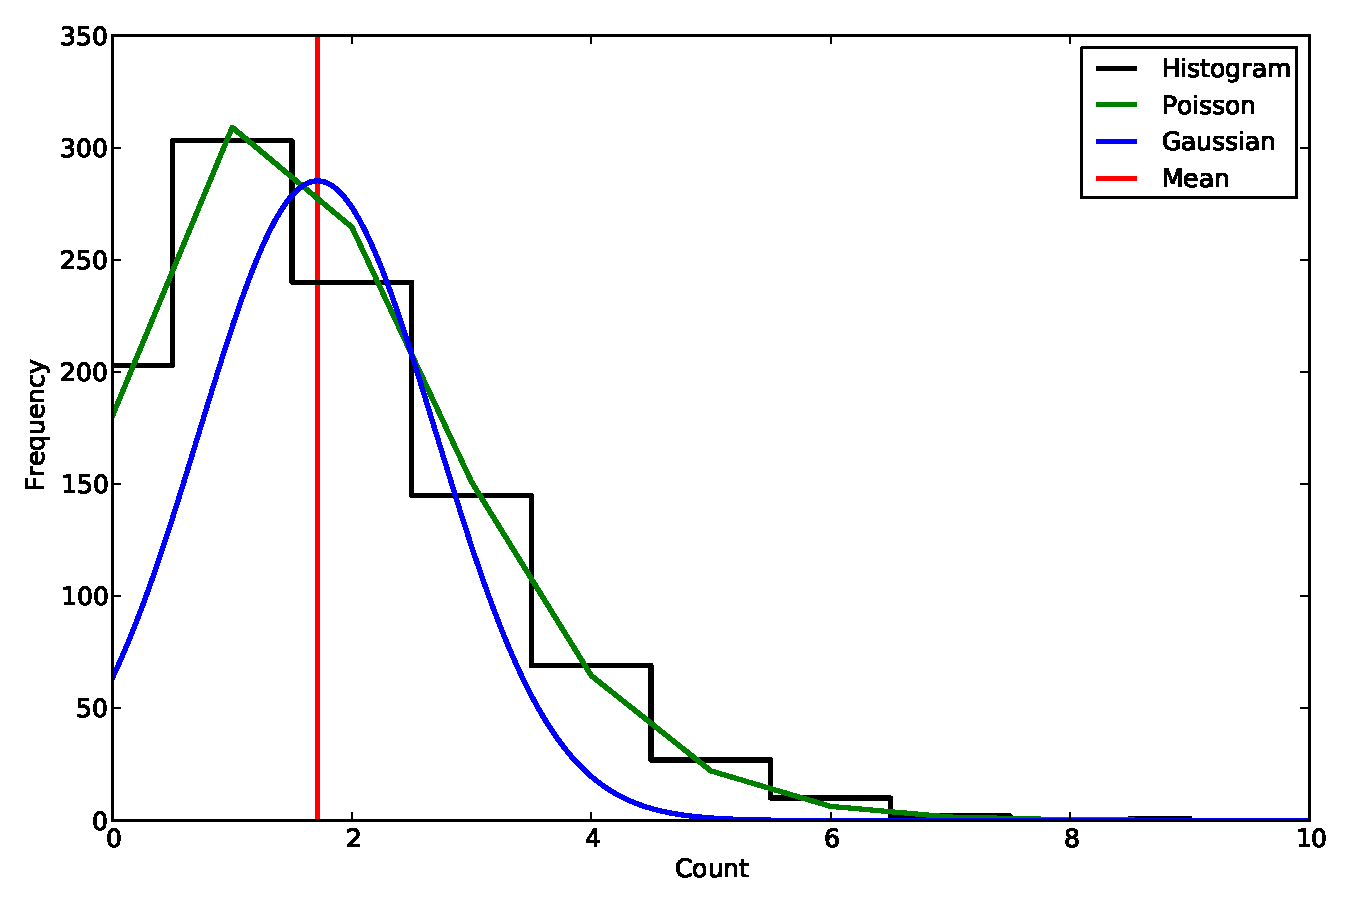
\includegraphics[angle=0,height=9cm,width=15.5cm]{graphs/Hist_distribution_small.pdf}
\caption{Histogram of data number 10 from Table \ref{table:dataset} with 1000 samples and time interval as 0.001. Here blues line is gaussian distribution, green is poisson distribution and red line indicated the mean value}
\label{fig:poisson}
\end{figure}

\begin{figure}[H]
\centering
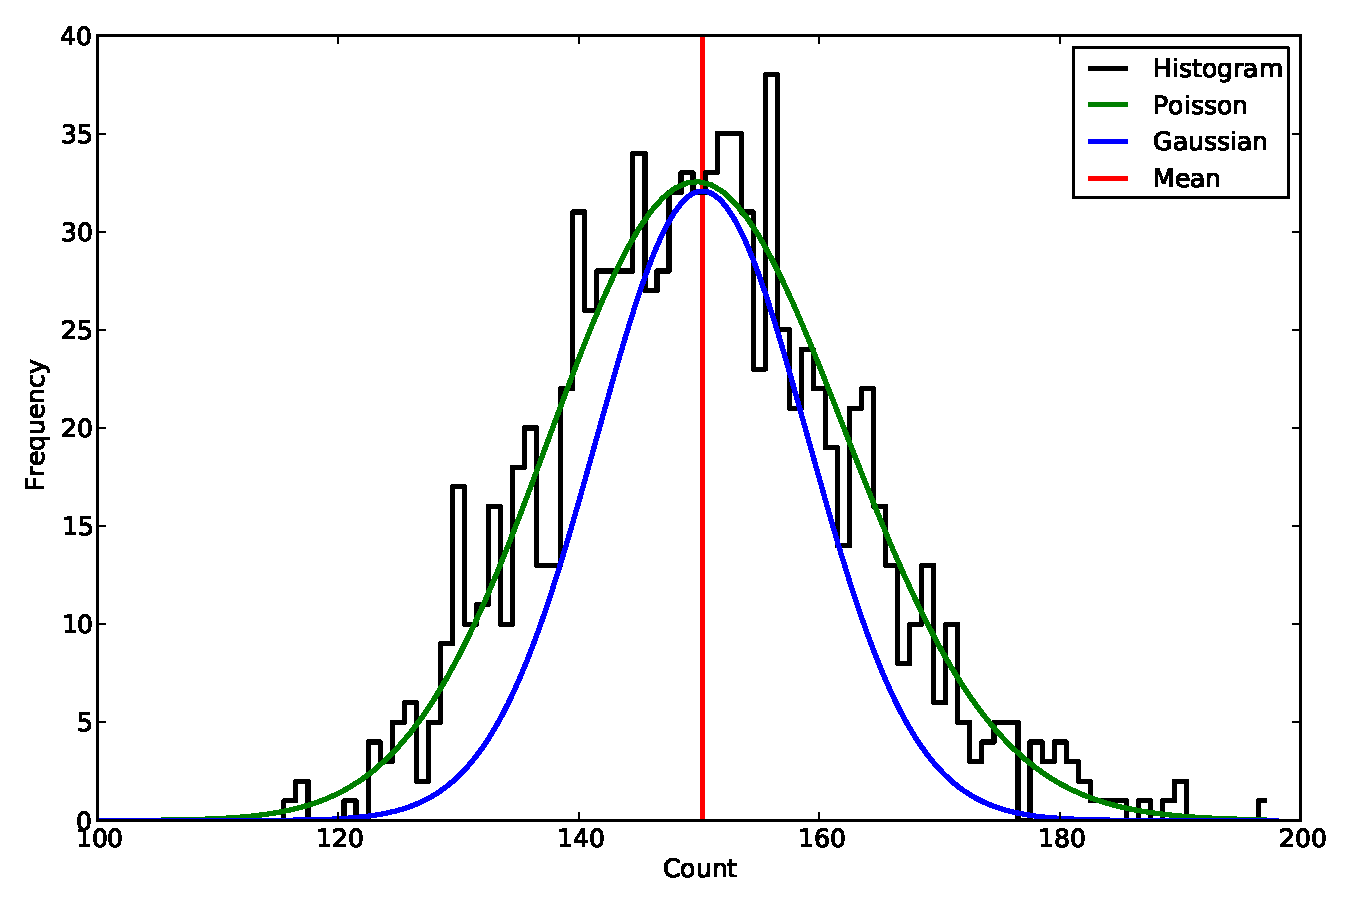
\includegraphics[angle=0,height=9cm,width=15.5cm]{graphs/Hist_distribution_big.pdf}
\caption{Histogram of data number 11 from Table \ref{table:dataset}with 1000 samples and time interval as 0.1. Here blues line is gaussian distribution, green is poisson distribution and red line indicated the mean value}
\label{fig:gaussian}
\end{figure}
%~~~~~~~~~~~~~~~~~~~~~~~~~~~~~~~~~~~~~~~~~~~~~~~~~~~
The two figures (Figure 7 and 8) two data with 1000 number of samples but different time interval: 0.001s and 0.01s, respectively. There is histogram of the data in black and mean in red on each plot. Poisson and Gaussian distribution on the plots are multiplied by 1000 to obtain correct scaling for comparing with histogram. One of the main thing to notice in these two graph is that for smaller time interval gaussian distribution (by Equation 4) does not right the histogram, however it does for the larger time interval. Poisson distribution (by Equation 3) fits both the histograms. This further proves that data collected correlates with poisson distribution. Gaussian is good approximate, if the time interval of data is large, as in Figure 8.  

%#######################  MOM and SDOM
\subsection{Exploring mean of mean and standard deviation of mean}
\label{sec:MOM_SDOM}

Data number 12 - 22 from Table \ref{table:dataset} was used to calculate the mean of mean (MOM) using Equation \ref{eq:mean} twice and standard deviation of mean (SDOM) using Equation \ref{eq:mean} and  \ref{eq:SD}. This was then plotted in count vs. number of samples plot. 

The Figure \ref{fig:task9} also have a theoretical graph, which was derived by the following method. For poisson distribution variance (standard deviation squared) is same as mean value ($\mu$) of the data as explained in Section \ref{sec:meanandvariance}. Therefore, the standard deviation of poisson distribution is $\sigma = \sqrt{\mu}$. And for expected error of mean, the formula is $\frac{\sigma}{\sqrt{N}} $ \citep{error}. Combining these two we get:

\begin{equation}
\label{eq:TSD}
\sigma_{exp} = \sqrt{\frac{\mu}{N}},
\end{equation}

where $\mu$ is the mean and $N$ is number of samples for one data. These value was for each set of data. To get $\sigma_{exp}$ for each number of samples. The mean of $\sigma_{exp}$ for a corresponding number of sample was taken using Equation \ref{eq:mean}. This is then the theoretical standard deviation representing poisson distribution. 

%~~~~~~~~~~~~~~~~~~~~~~~~~~~~~~~~~~~~~~~~~~~~~~~~~~~
\begin{figure}[H]
\centering
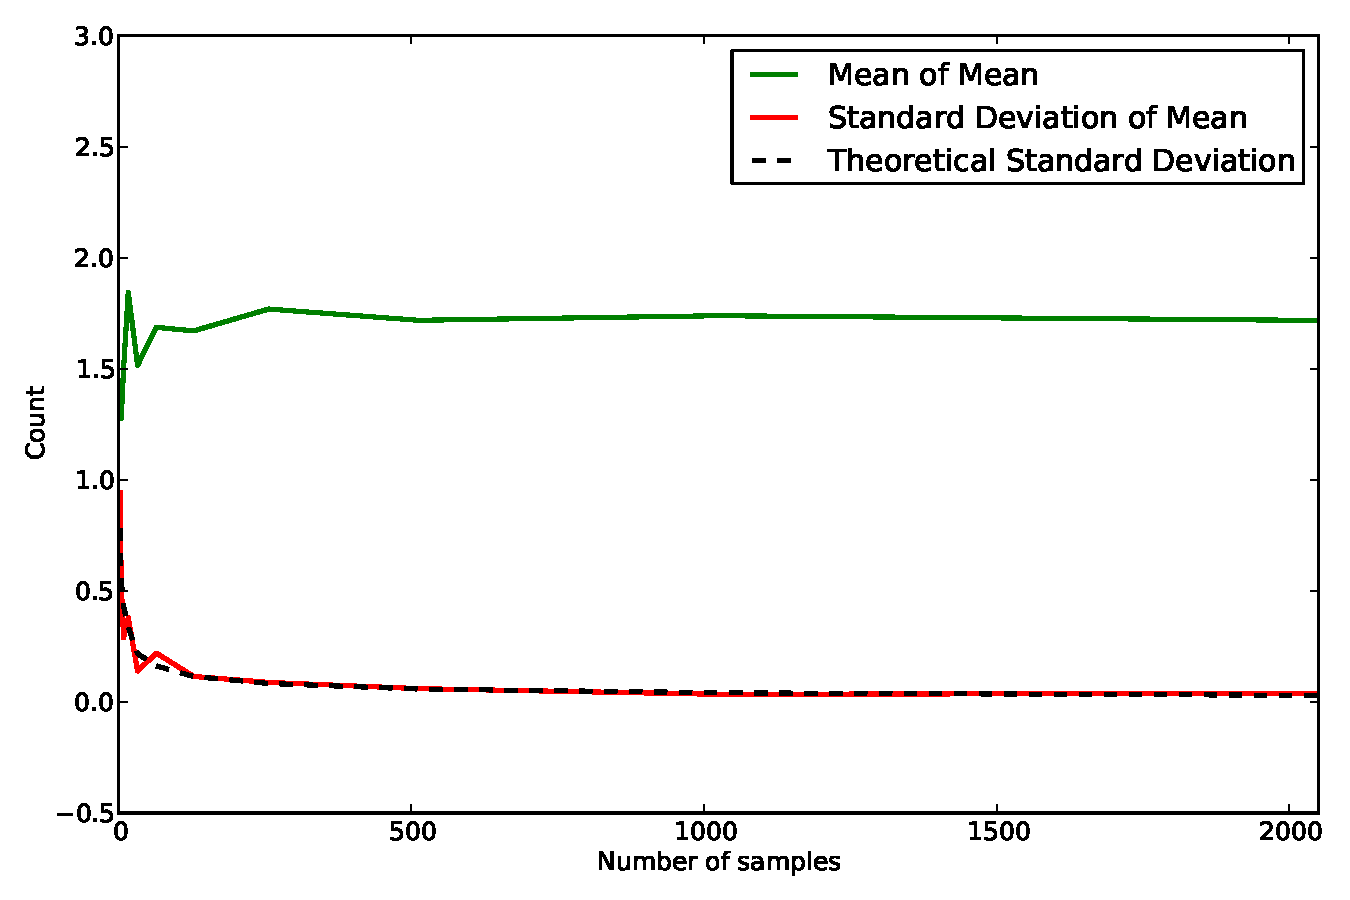
\includegraphics[angle=0,height=10cm,width=15.5cm]{graphs/task9.pdf}
\caption{Plot of mean of mean and standard deviation of mean vs. number of samples. This plot also show the theoretical prediction of the mean by Equation \ref {eq:TSD}.}
\label{fig:task9}
\end{figure}
%~~~~~~~~~~~~~~~~~~~~~~~~~~~~~~~~~~~~~~~~~~~~~~~~~~~

It can be induced from Figure \ref{fig:task9} that as the number of samples increases, then MOM converge to a certain value and SDOM get closer to zero. Therefore with high number of samples, not only more accurate MOM can be obtained but also the error can be reduced. However, having too big number of samples does not make a huge difference because the two values stay very much consistent. And, it is clear in the figure that the theoretical standard deviation fits the SDOM very well. Therefore, to improve the precision of a measurement of mean by factor of 2, number of samples should be increased by the 4. This can be induced from Equation \ref {eq:TSD}. 

%######################### Conclusion
\section{Conclusion}
Photons detected using PMT based on different number of samples and time intervals show high correlation with poisson distribution. Mean value is equal to the variance for all data set. However, at larger time interval, the data set is also approximated to gaussian distribution, but not completely. It also shown that at larger number of samples the MOM approaches a certain value and SDOM approaches zero. This also fits with theoretical standard deviation calculated by using poisson statistics and error propagation. 

\bibliographystyle{plain}
\bibliography{references.bib}
\end{document}
